\documentclass{article} % For LaTeX2e
\usepackage{nips13submit_e,times}
\usepackage{hyperref}
\usepackage{url}
\usepackage{graphicx}
\usepackage{enumitem,amsmath,amssymb}
%\documentstyle[nips13submit_09,times,art10]{article} % For LaTeX 2.09


\title{Playlist Title Generation Using Sequence to Sequence}


\author{
    Sof\'ia Samaniego de la Fuente \\
    Department of Statistics \\
    Stanford University \\
    \texttt{sofiasf@stanford.edu}
    \AND
    Advisor: Richard Socher 
}

% The \author macro works with any number of authors. There are two commands
% used to separate the names and addresses of multiple authors: \And and \AND.
%
% Using \And between authors leaves it to \LaTeX{} to determine where to break
% the lines. Using \AND forces a linebreak at that point. So, if \LaTeX{}
% puts 3 of 4 authors names on the first line, and the last on the second
% line, try using \AND instead of \And before the third author name.

\newcommand{\fix}{\marginpar{FIX}}
\newcommand{\new}{\marginpar{NEW}}

\nipsfinalcopy % Uncomment for camera-ready version

\begin{document}


\maketitle

\begin{abstract}
In this project we propose a model that generates the name of a playlist given information about its tracklist. 
We first use a standard sequence-to-sequence model with unidirectional single-layer LSTM cells for both the encoder and the decoder and GloVe embedding initialization. 
We then add drop-out for regularization and introduce an attention mechanism to establish alternative connections between relevant words in song titles and playlist names.  
%We then add drop-out for regularization, extend our encoder and decoder cells to multi-layer LSTMs and introduce an attention mechanism to establish alternative connections between relevant words in song titles and playlist names.  
Finally, we provide an interactive console that generates playlist name suggestions given an input tracklist, which could serve as a useful automated suggestion system for digital music services users.   
\end{abstract}

\section{Introduction}
\label{sec:intro}

Coming up with an original and catchy title for a playlist is most definitely a challenging task. %, even for humans.
In this project we propose a neural model dedicated to making the name search easier for those in the hunt for the perfect playlist title. 
In particular, we attempt to construct a network that builds an internal representation of the names of the tracks included in a playlist and then uses natural language techniques to generate a title that could be close to what a human might devise. 

Generating a playlist name is somewhow related to the task of creating a condensed representation of an input text; that is, to the task of summarization.
Specifically, this problem is similar to abstractive summarization, as a title generally captures the gist of a playlist without explicitly using segments of the song titles included in it, as an extractive method does. 
We hence approach this problem through a neural sequence-to-sequence model, the most viable and promising approach for abstractive summarization available at present. 
These models, first introduced by Sutskever et al.~\cite{sutskever2014sequence}, typically use an LSTM cell to map an input sequence to a vector of fixed dimensionality and then another LSTM to decode the target sequence from the vector. 
They have proven successful in a variety of tasks such as machine translation, question answering, bot interaction, and automatic summarization.  

%Many challenges lie in this project. 
There are numerous challenges to overcome in this project.
In particular, it is hard to quantify how well a title conveys the relevant information of a playlist, aspects of which may not appear in the input text. 
Furthermore, deciding whether a playlist name is ``good" is a highly subjective task that is difficult even for humans, so coming up with a good automatic evaluation metric is particularly challenging. 
To evaluate the final performance of our model, we use both a quantitative measure, namely the ROUGE score, as proposed in NITS's annual Document Understanding Conferences~\cite{he2008rouge}, and a qualitative one, namely the analysis of example results. 

The rest of the paper is organized as follows. 
In Section~\ref{sec:bg} we discuss relevant literature for this project.
In particular, we provide a brief review on previous work in sequence-to-sequence models for abstractive summarization. 
We note, however, that, to our knowledge, no one has ever proposed the specific task of generating playlist titles using neural natural language processing techniques. 
In Section~\ref{sec:app}, we delineate the architecture of our standard and extended neural models. 
We then describe and analize our dataset and summarize our experimental results in Section~\ref{sec:exp}. 
We show that our approach yields in human-like and creative results for most input playlists. 
Finally, we conclude the project with ideas for future work in Section~\ref{sec:conc}.   

\section{Background}
\label{sec:bg}
Automatic summarization refers to the process of creating a condensed, fluent, and accurate representation of an original input text using natural language processing techniques.
While this problem has long been a research topic of great interest in computer science, in recent years this interest has spiked due to an increase in availability of text data from a variety of sources, including a huge amount of online articles and documents.
There are two general approaches for this problem: extraction and abstraction. 
Extractive methods work by assembling summaries from important sections taken verbatim from the source text; meanwhile, abstractive methods, which will be our main focus, aim to convey relevant information by generating novel words and phrases which may or may not appear in the source text~\cite{allahyari2017text}.

In 2015, Rush et al.~\cite{rush2015neural} proposed a local attention-based model that generates each word of the summary conditioned on an input sentence. 
Their model achieved significant performance gains on the DUC-2004 evaluation dataset, consisting of 500 document-summary pairs.   
Nallapati et al.~\cite{nallapati2016abstractive} modeled abstractive text summarization using attentional encoder-decoder RNNs in 2016 and outperformed several state-of-the-art results on two different datasets: the DUC-2004 corpus and the CNN/Daily Mail corpus.
Finally, See et al.~\cite{see2017get} proposed an extension to the standard sequence-to-sequence architecture for abstractive text summarization in 2017.
Their model tackled two shortcomings of the standard architecture by introducing the use of a hybrid pointer generator network to aid in the liable reproduction of factual details and coverage to discourage repetition. 
They outperformed the current abstractive state-of-the art by over $2$ ROUGE points in the CNN/Daily Mail dataset.

Text summarization is without a doubt a non-trivial task for computers, since this process implies the use of human knowledge and language capability, both of which computers lack. 
While a lot of progress has been made in this area with the recent success of neural models and other data driven approaches, this remains a very challenging task and attaining high levels of abstraction remains an open research question. 
 
\section{Methods}
\label{sec:app}
In this section we describe our standard baseline sequence-to-sequence model, the regularized version using dropout, and the extended attention-based model, modeled off the attention mechanism introduced by Bahdanau et al. in 2015~\cite{bahdanau2014neural}. 

\subsection{Standard sequence-to-sequence model}
\label{sec:seq2seq}

Our baseline model, depicted in Figure~\ref{fig:architectures}, is similar to that presented by Luong et al.~\cite{luong17} in their Neural Machine Translation (seq2seq) Tutorial.

We start by tokenizing the words in the song names of our playlists and their corresponding titles into a sequence of tokens which roughly correspond to words.
We will represent the tokens of the tracklist of each playlist as a sequence of integers
\[
x_1, x_2, \dots x_T
\]
where $T$ is the arbitrary input length, each $0 \le x_t \le |V|$ is the index of a token in the vocabulary, and $|V|$ is the vocabulary size. 
The top $|V|$ most frequent tokens in our data are treated as unique, while all other are converted to an ``unknown" token and get the same embedding. 

These tokens are fed into the encoder (a single-layer unidirectional LSTM), who looks for the corresponding word representations $E_{x_t}$ in the embedding matrix $E \in \mathbb{R}^{|V|\times d}$ (embedding layer) and then uses them as input to produce a sequence of hidden states $h_1, h_2, \dots, h_T$.

On each step $t$, the decoder (also a single-layer unidirectional LSTM) receives the last hidden state of the encoder $h_t$ and the word token of the previous word (the previous word of the target playlist title during training, the previous word emitted greedily by the decoder during test time).
The decoder then looks up the corresponding embedding and uses it as input along with the encoding of the source tracklist to generate a hidden state $s_t$, which it then transforms into a logit vector of dimension $|V|$ (projection layer). 
Finally, the decoder produces a playlist title conditioned on the encoding of its tracklist by finding the maximum logit value of its outputs at each time step. 

\begin{figure*}
    \centering
    \begin{minipage}[b]{.49\linewidth}
        \centering
            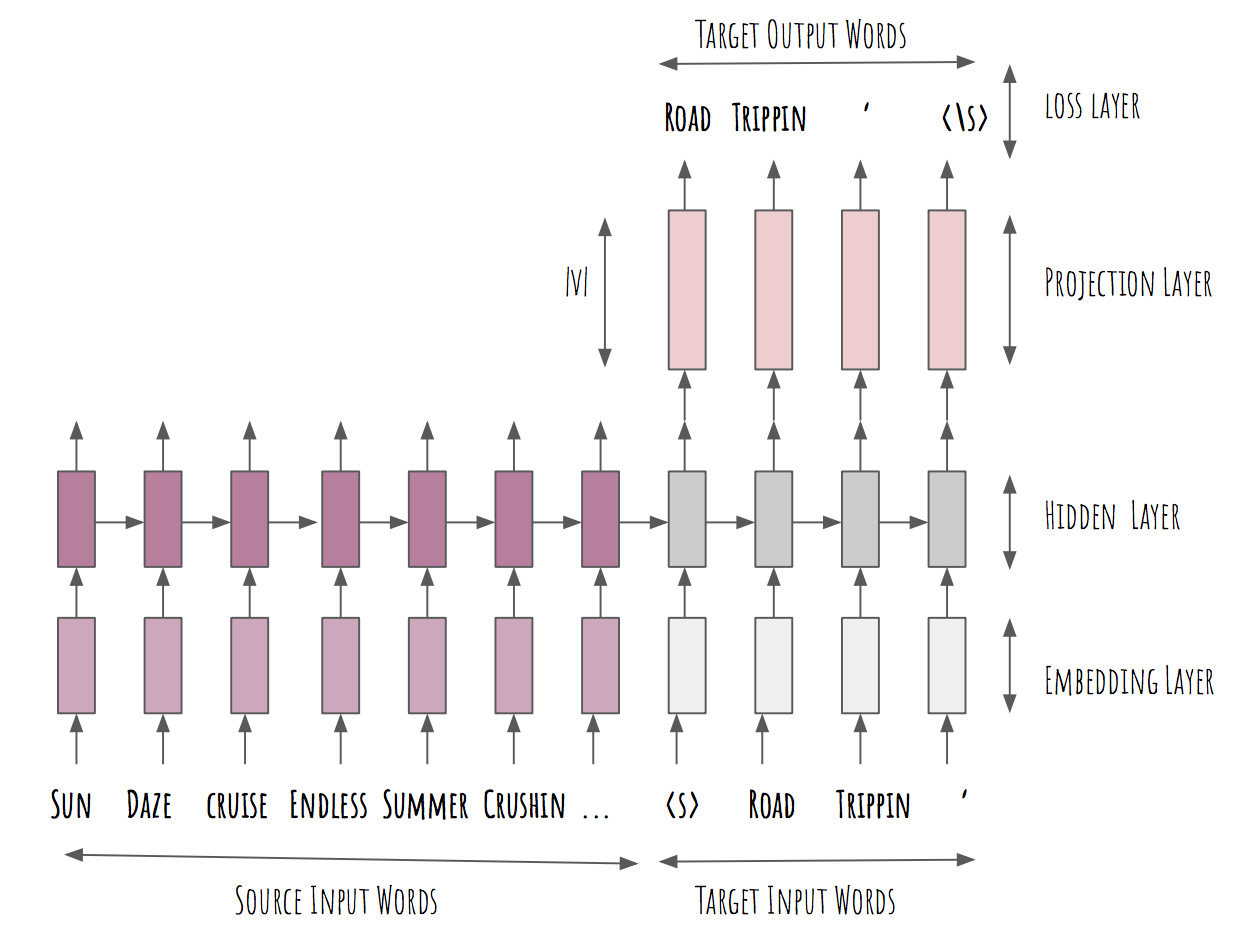
\includegraphics[trim={0.3cm 0cm 0cm 1cm}, clip, width=\textwidth]{train-arch.png}
        \label{fig:standard_arch}
    \end{minipage}%
    \hfill%
    \begin{minipage}[b]{.49\linewidth}
    \centering
        \centering
            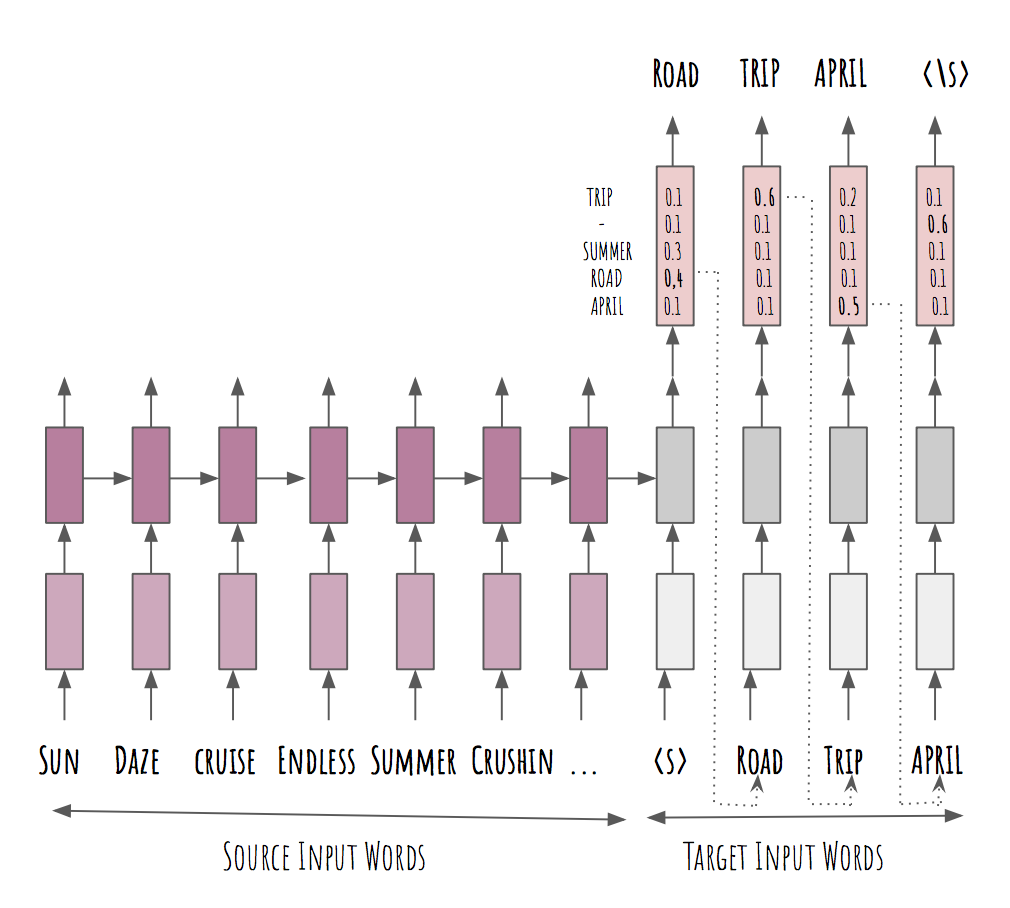
\includegraphics[trim={0cm, 0.5cm, 0cm, 2cm}, clip, width=\textwidth]{infer-arch.png}
        \label{fig:test_standard_arch}
    \end{minipage}\\[-7pt]
    \begin{minipage}[t]{.45\linewidth}
        \caption{Standard sequence-to-sequence network architecture at train time.
        During training, the decoder receives as input the sequence of tokens in the target playlist name with an additional start-of-sentence token appended on the right.
        Here, `\textless s\textgreater' marks the start of the decoding process while `\textless$\backslash$ s\textgreater' tells the decoder to stop.}
    \end{minipage}%
    \hfill%
    \begin{minipage}[t]{.45\linewidth}
        \caption{Standard sequence-to-sequence network architecture at test time. Here, the decoder is initially fed a starting symbol to indicate the start of the decoding process; subsequently, its own output is fed as its next step's input. The process continues until the end-of-sentence marker is produced or we reach the maximum number of iterations.}
    \end{minipage}%
\label{fig:architectures}
\end{figure*}


%\begin{figure}[h]
%\begin{center}
    %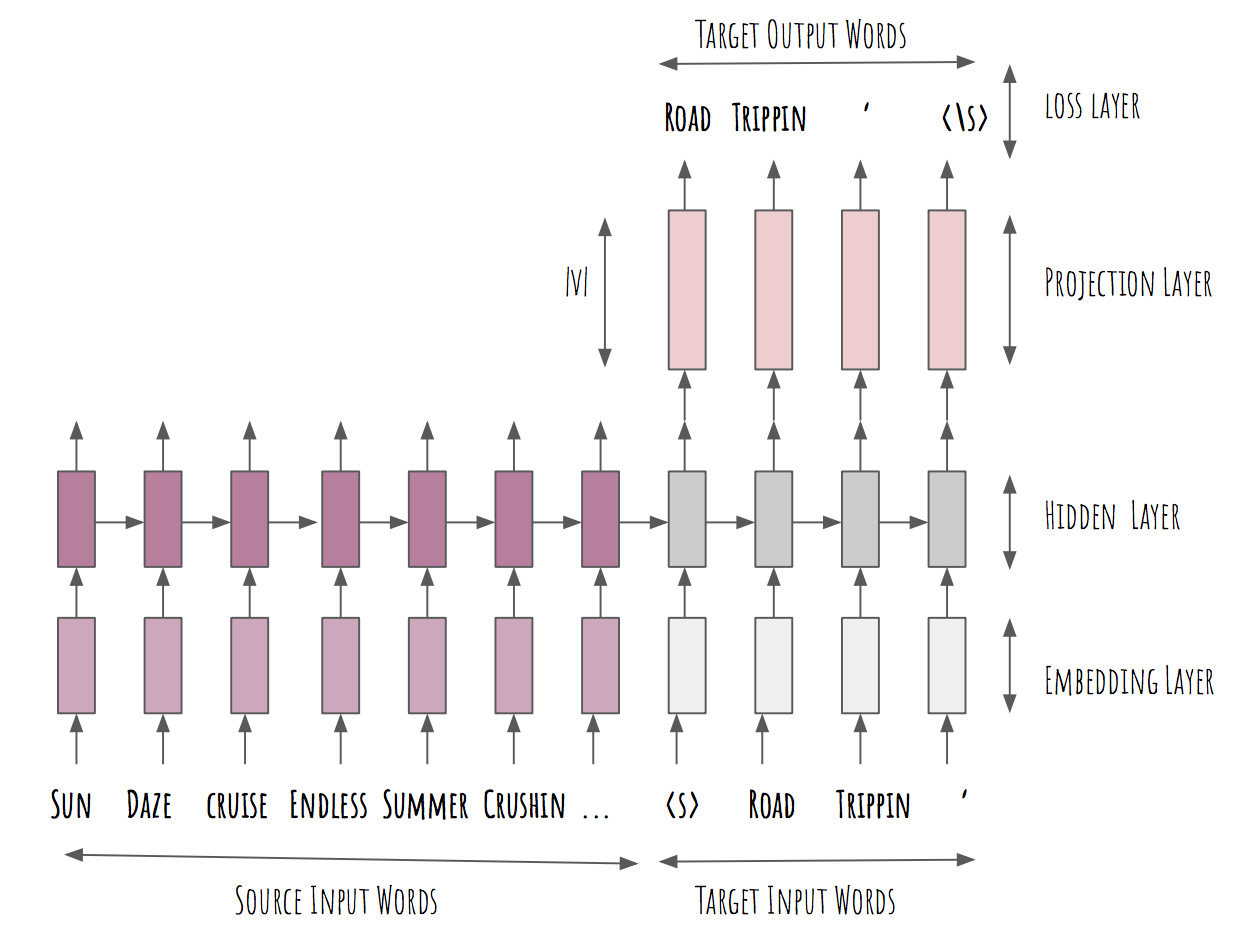
\includegraphics[trim={0cm 0cm 0cm 1cm}, clip, width=0.78\textwidth]{train-arch.png}
%\end{center}
%\caption{Standard sequence-to-sequence network architecture at train time. 
%Here, `\textless s\textgreater' marks the start of the decoding process while `\textless$\backslash$ s\textgreater' tells the decoder to stop.}
%\label{fig:standard_arch}
%\end{figure}


%\begin{figure}[ht]
%\begin{center}
    %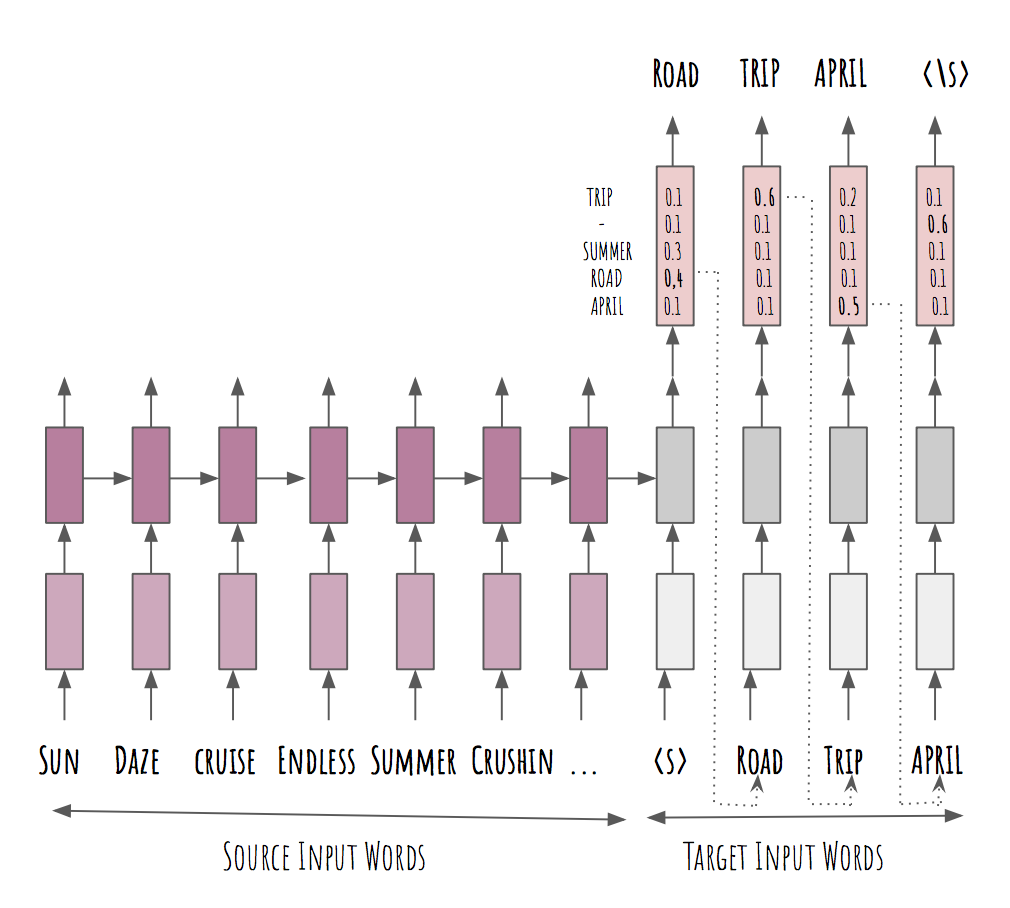
\includegraphics[trim={0cm, 0cm, 0cm, 2cm}, clip, width=0.68\textwidth]{infer-arch.png}
%\end{center}
%\caption{Standard sequence-to-sequence network architecture at test time. Here, the decoder is initially fed a starting symbol to indicate the start of the decoding process; subsequently, its own output is fed as its next step's input. The process continues until the end-of-sentence marker is produced or we reach the maximum number of iterations.}
%\label{fig:test_standard_arch}
%\end{figure}


During training, the loss function is a weighted softmax cross-entropy loss, where the weights are used to mask padding positions outside of the target sequence lengths with values of zero. In particular, at each timestep $t$, 
\[
    J^{(t)}(\theta) = -\log(P(y_t))
\]
where $y_t$ is the target token at that timestep and $P$ is the probability distribution produced by the decoder over all words in the vocabulary; meanwhile, the overall loss for the whole playlist title is given by 
\[
    J(\theta) = \frac{1}{M}\sum_{t=0}^{M} m^{(t)}J^{(t)}(\theta),
\]
where $m^{(t)}$ is a masking vector which is $1$ for all $t \le T^*$ and $0$ for all $t > T^*$ where $T^{*}$ is the length of the target sequence and $M$ is the maximum output length. 

\subsection{Regularized sequence-to-sequence model}
This model is identical to the standard sequence-to-sequence network described in Section~\ref{sec:seq2seq}, except that we additionally regularize our network by applying Dropout~\cite{srivastava2014dropout} to avoid overfitting.
This process amounts to creating an ensemble of smaller networks that share the same weights. 

We drop the same network units (inputs, outputs, and recurrent connection) at each time step to avoid an aggregation of the dropout masks that could amplify the noise and drown down the signal of our input, as suggested by Gal et al.~\cite{gal2016theoretically}. 
%We introduce dropout only to the output of the encoder and the decoder LSTM cells to avoid an aggregation of the dropout masks that could amplify the noise and drown down the signal of our input~\cite{zaremba2014recurrent}. 
%We do not apply dropout at test time. 
At test time, all neurons are kept to combine all the smaller networks into a single one and the activationas are scaled by the dropout probability to ensure the expected value is the same as the actual output.  

\subsection{Attentional sequence-to-sequence model}
We introduce an attention mechanism to our original sequence-to-sequence network, which relieves the encoder from the burden of having to encode all information in the source sequence into a fixed length vector~\cite{bahdanau2014neural} by allowing the decoder a glimpse into the hidden states of the encoder.
\begin{figure}[h]
\centering
\includegraphics[clip, width=0.7\textwidth]{attn}
\caption{Toy attention visualization. Darker tones denote higher attention score.}
\label{img:attn}
\end{figure}
%We introduce two additional modifications to our original sequence-to-sequence network: attention and an additional layer. 
%The attention mechanism relieves the encoder from the burden of having to encode all information in the source sequence into a fixed length vector~\cite{bahdanau2014neural} by allowing the decoder a glimpse into the hidden states of the decoder.

The attention distribution is calculated as follows:
\begin{align*}
    e_i^{(t)} &= v_a^\top\mbox{tanh}(W_1h_i + W_2s_t) \\
    d^{(t)} &= \mbox{softmax}(e^{(t)}),
\end{align*}
where $v_a$, $W_1$, and $W_2$ are learnable parameters. 
This attention distribution is then used to produce the context vector $c_t$, a linear combination of the source hidden states
\[
c_t = \sum_{i}d_i^{(t)}h_i.
\]
Finally, the context vector is combined with the current target hidden state to yield the final attention vector
\[
a_t = f(c_t, h_t) = \mbox{tanh}(W_c[c_t; h_t]),
\] 
which is fed as an input to the next time step.

We try two variants of this attentional model, one with a unidirectional RNN and the other with a bidirectional RNN for the encoder.
%In addition to the attention mechanism, we add an additional layer to both our encoder and decoder LSTM cells to allow for more complex representations of our inputs.

\section{Experiments}
\label{sec:exp}
In this section we: (1) describe the dataset used for our experiments along with some exploratory analysis on coverage, (2) report the choice of final vocabulary used in our model, (3) delineate the model configuration of our experiments, (4) describe the metrics used for performance evaluation, and (5) layout our final results. 

\subsection{Dataset and Vocabulary}
\label{sec:data}

We evaluate our proposed models on the Million Playlist Dataset\footnote{Official website hosted at \href{https://recsys-challenge.spotify.com}{https://recsys-challenge.spotify.com}}, recently released by Spotify as part of its 2018 RecSys Challenge.
It comprises a set of $1,000,000$ playlists that have been created by Spotify users along with a variety of features, including playlist name, description, timestamp when the playlist was last updated, and an array of information about each track in the playlist (track name, artist, album name, duration, and position in the playlist).
To simplify our analysis, we work only with playlist names and their corresponding tracklist. 

\subsubsection{Summary Statistics and Coverage}
\label{sec:stats}

There are $92,944$ unique titles among our playlists. Tables~\ref{tab:tp} and~\ref{tab:tt} show the top playlist titles and tracks with their corresponding count in the full dataset, prior to any processing.

\begin{table}[ht]
\begin{minipage}[b]{0.4\linewidth}
\centering
    \begin{tabular}{rl}
    \multicolumn{1}{r}{\bf Playlist name} &  \multicolumn{1}{l}{\bf Count (K)}  \\
    \hline \\
    Country & 10  \\
    Chill & 10 \\
    Rap & 8.5\\
    Workout & 8.5\\
    Oldies & 8.1\\
    Christmas & 8.0 \\
    Rock & 6.8\\
    Party & 6.2\\
    Throwback & 5.9\\
    Jams & 5.1\\ 
    \end{tabular}
    \caption{Top playlist names}
    \label{tab:tp}
\end{minipage}\hfill
\begin{minipage}[b]{0.6\linewidth}
\centering
    \begin{tabular}{rl}
    \multicolumn{1}{r}{\bf Song name and artist}& \multicolumn{1}{l}{\bf Count (K)}\\
    \hline \\
    HUMBLE. by Kendrick Lamar & 46.6 \\
    One Dance by Drake & 43.4 \\
    Broccoli (feat. Lil Yachty) by DRAM & 41.3 \\
    Closer by The Chainsmokers & 41.1\\
    Congratulations by Post Malone & 40.0 \\
    Caroline by Aminé & 35.2\\
    iSpy (feat. Lil Yachty) by KYLE & 35.1\\
    Bad and Boujee (feat. Lil Uzi Vert) by Migos & 35.0 \\
    Location by Khalid& 35.0 \\
    XO TOUR Llif3 by Lil Uzi Vert & 34.9 
    \end{tabular}
    \caption{Top tracks}
    \label{tab:tt}
\end{minipage}
\end{table}


We analyze the word coverage of our dataset to decide the size of our vocabulary. 
As shown in Table~\ref{tab:wc}, we find that the top $20,000$ most frequent words account for over $98\%$ of all the words in the dataset, including words in the tracklists and playlist names. 
We hence decide to treat only the top $|V| = 20,000$ of words as unique and convert all other words to an unknown token.

We then filter out playlists with unknown tokens in their title, after which we are left with a total of $885,303$ playlist name-tracklist pairs. 
We split our dataset into train, validation, and test sets using an $85\%-15\%-5\%$ split, which yields in $708,243$ training pairs, $132,795$ validation pairs, and $44,265$ test pairs.

\begin{table}[!h]
\begin{minipage}[b]{0.5\linewidth}
\centering
    \begin{tabular}{ccc}
    \multicolumn{1}{c}{\bf Top $k$ words}  &\multicolumn{2}{c}{\bf Coverage}\\
                                           & \# words (M) & \% 
    \\ \hline \\
    $1,000$ & $166.8$ & $73.8$\\
    %$2,000$ & $187.1$ & $82.7$\\
    $5,000$ & $207.6$ & $91.8$\\
    $10,000$ & $217.1$ & $96.0$\\
    $20,000$ & $221.1$ & $98.2$\\
    $30,000$ & $223.7$ & $99.0$\\
    %$40,000$ & $224.5$ & $99.3$\\
    \end{tabular}
    \caption{Word coverage}
    \label{tab:wc}
\end{minipage}\hfill
\begin{minipage}[b]{0.5\linewidth}
\centering
    \begin{tabular}{ccc}
    \multicolumn{1}{c}{\bf Top $k$ titles}  &\multicolumn{2}{c}{\bf Coverage}\\
                                            & \# playlists (K) & \% 
    \\ \hline \\
    $1$ & $10.0$ & $1.6$\\
    %$5$ & $45.1$ & $7.6$\\
    $10$ & $77.1$ & $13.0$\\
    $20$ & $119.6$ & $20.2$\\
    $50$ & $193.1$ & $32.6$\\
    $100$ & $255.2$ & $43.1$\\
    \end{tabular}
    \caption{$1$-word playlist title coverage}
    \label{tab:tc}
\end{minipage}
\end{table}

Table~\ref{tab:tc} shows the playlist coverage of the top 100 playlist names; that is, the percentage of total playlists with one-word names in the top $100$ playlist titles.
We conclude that there is enough variation in our targets not to treat this problem as a classification task.
However, for completeness, we ran a BOW model, a logistic regression, and an LSTM model with an additional soft-max layer to classify the $119,573$ playlists with single-word names in the top $20$ titles. 
These models yielded in accuracies of $0.564$, $0.546$, and $0.547$, respectively. 
All of these accuracies are significantly higher than the $0.01$ accuracy that a majority-vote model (predicting the top title \emph{Country} for all playlists) would have resulted on. 
We can hence conclude there is enough signal in our input data achieve a good performance on our title generating task.

Finally, the mean number of words our tracklists is $224.9$, while the number of words in the playlist titles ranges from $1$ to $14$, with around $63\%$ of the playlist having single-word titles and over $99\%$ less than $5$ words in their title. 
We will use this information to decide the maximum input and output sequence lengths in our models.

\subsection{Experiment Setup}
We implemented our model using Tensorflow~\cite{tensorflow2015-whitepaper}.
For all our experiments, our model has $256$-dimensional hidden states and $100$-dimensional word embeddings.
We tokenize using the PTBTokenizer provided by the Stanford Natural Language Processing Group.
We use pretrained GloVe~\cite{pennington2014glove} vectors to initialize our word embeddings and treat them as trainable parameters in our model.
We train using Adam with learning rate $0.0025$. 
For our standard sequence-to-sequence model, we also try learning rates of $0.001$ and $0.005$.
We use gradient clipping with a maximum gradient norm of $5$. 
In the regularized version of our model, we use drop probability of $0.2$.
In all our other models we do not use any form of regularization, but we use ROUGE in the validation set to implement early stopping. 

During training and at test time we truncate the tracklist length to $200$ tokens and limit the playlist name to $6$ tokens (including the start- and end-of-sentence tokens for the decoder inputs and targets).
We chose these values based on the summary statistics presented in Section~\ref{sec:stats}.

We train our baseline sequence-to-sequence model and the regularized model for a limit of $25$ epochs and our final attentional models for a limit of $30$ epochs. 
Training of our final model took $24$ hours on a Tesla M60 GPU with batch size of $64$. At test time our playlist titles are produced using Greedy decoding.

\subsection{Evaluation Metrics}
\label{sec:metric}

We evaluate our model reporting the $F_1$ scores for ROUGE\footnote{The acronym ROUGE stands for Recall-Oriented Understudy for Gisting Evaluation.}-$2$, which corresponds to bi-gram overlap between the titles generated by our model and the true labels of our test dataset. 
We obtain our ROUGE scores using Google's implementation found \href{https://github.com/google/seq2seq/blob/master/seq2seq/metrics/rouge.py}{here}~\cite{Britz:2017}.

Since this metric could lead to bad scores for creative titles and due to the high subjectivity of this task, we also provide a qualitative analysis of example title names produced by our models.

\subsection{Results}
\label{sec:results}
In this section we: (1) describe the tuning process that lead to our final learning rate choice, (2) provide a quantitative assessment of our experimental results based on the metric presented in Section~\ref{sec:metric}, and (3) lay out a qualitative evaluation of our models through the analysis of the titles generated for the playlists in our test set.  

\subsubsection{Initial hyper-parameter tuning}
We run our standard sequence-to-sequence architecture decribed in Section~\ref{sec:seq2seq} for different values for the learning rate, namely $\eta \in \{0.001, 0.0025, 0.005\}$. 
Figure~\ref{fig:tuning} shows the corresponding train and validation ROUGE-$2$ curves.   

\begin{figure*}[!h]
    \centering
    \caption{Train and validation $F_1$ scores for $2$-ROUGE for different learning rates}
    \begin{minipage}[b]{.3\linewidth}
        \centering
        \includegraphics[width=\linewidth]{rouge001.pdf}
    \end{minipage}%
    \hfill%
    \begin{minipage}[b]{.3\linewidth}
        \centering
        \includegraphics[width=\linewidth]{rouge0025_2.pdf}
    \end{minipage}%
    \hfill%
    \begin{minipage}[b]{.3\linewidth}
        \centering
        \includegraphics[width=\linewidth]{rouge005.pdf}
    \end{minipage}\\[-7pt]
    \begin{minipage}[t]{.3\linewidth}
        \caption{$\eta = 0.001$}\label{fig:awesome_image1}
    \end{minipage}%
    \hfill%
    \begin{minipage}[t]{.3\linewidth}
        \caption{$\eta = 0.0025$}\label{fig:best_rouge}
    \end{minipage}%
    \hfill%
    \begin{minipage}[t]{.3\linewidth}
        \caption{$\eta = 0.005$}\label{fig:awesome_image3}
    \end{minipage}%
\label{fig:tuning}
\end{figure*}

%\begin{figure}[!htb]
%\caption{Train and validation $F_1$ scores for $2$-ROUGE for different learning rates}
%\minipage{0.30\textwidth}
  %\includegraphics[width=\linewidth]{rouge001.pdf}
  %\caption{$\eta = 0.001$}\label{fig:awesome_image1}
%\endminipage\hfill
%\minipage{0.30\textwidth}
  %\includegraphics[width=\linewidth]{rouge0025_2.pdf}
  %\caption{$\eta = 0.0025$}\footnote{Note that we ran this model for $5$ extra epochs to allow the train loss to plateau.}\label{fig:best_rouge}
%\endminipage\hfill
%\minipage{0.30\textwidth}%
  %\includegraphics[width=\linewidth]{rouge005.pdf}
  %\caption{$\eta = 0.005$}\label{fig:awesome_image3}
%\endminipage
%\label{fig:tuning}
%\end{figure}
We observe that $\eta = 0.005$ is too high, since the training ROUGE plateaus at a low value of approximately $0.25$. 
On the other hand, we see that the training ROUGE increases roughly linearly for the first $15$ epochs with $\eta = 0.001$ and then plateaus, which suggests this learning rate is too small. 
Meanwhile, when $\eta = 0.0025$\footnote{Note that we ran this model for five extra epochs to allow the train loss to plateau.}, the shape of the training ROUGE exhibits roughly logarithmic growth.

Further, the gap between the training and validation ROUGE scores is smallest when $\eta = 0.0025$, which suggests that this model will generalize best out of the three to unseen observations. 
Based on this analysis, we choose $\eta = 0.0025$ as a learning rate parameter for the rest of our experiments.     

\subsubsection{Quantitative Results}

Our results are shown in Table~\ref{tab:rouge}. 
Our best model scores achieve a $2$-ROUGE score of $42.1$ on the test set. 
We observe that adding drop-out does not results in an improvement with respect to our standard model.
We note that our network is small relative to our dataset and we are lowering its complexity further by introducing regularizartion.
Further, as shown in Figure~\ref{fig:best_rouge}, we were already doing very little overfitting; as a result, regularization hurt our model instead of helping.
Hence, we decide not to add dropout in the rest of our models and do early stopping based on $2$-ROUGE performance on the validation set instead.
Meanwhile, the introduction of an attention mechanism yields in a $4.6$ point increase in the test $2$-ROUGE score when the encoder is a unidirectional RNN. However, using a bidirectional RNN for the encoder results in a significantly lower ROUGE score, possibly because this model is too complex and has started fitting the error in the training set.   

\begin{table}[ht]
\begin{center}
\begin{tabular}{lc}
\multicolumn{1}{c}{\bf Model}  &\multicolumn{1}{c}{\bf $2$-Rouge $F_1$}\\ 
\hline \\
standard seq-to-seq & 37.5\\ 
standard seq-to-seq + dropout &  26.2\\ 
{\bf standard seq-to-seq + attention} & {\bf 42.1}\\
standard seq-to-seq + attention + bidirectional encoder & 30.4\\
%standard seq-to-seq + attention + extra layer & \\ 
\end{tabular}
\end{center}
\caption{Rouge $F_1$ scores on the test set. We note that we have no baselines from previous work to compare our results with, since, to our knowledge, no one has used this dataset for a similar task before.
However, for reference, the test ROUGE-$2$ $F_1$ scores for the models and baselines for abstactive summarization presented by See et al.~\cite{see2017get} range from $11.17$ to $17.70$. Our best model is the attentional sequence-to-sequence model with an unidirectional RNN for the encoder.}
\label{tab:rouge}
\end{table}

\subsubsection{Qualitative results}

We start by analyzing the playlists in which our model performs well in terms of ROUGE; that is, test examples where the bi-gram overlap between targets and predictions is high. 
In particular, we will analyze the examples in which our model predicts exactly the target playlist title. 

Figure~\ref{fig:correct} shows the target playlist titles that our best model predicted exactly on the test set more than $50$ times along with the number of times playlists with that title were ``classified" correctly. 

\begin{figure}[!hbt]
	\centering
		\includegraphics[width=0.6\textwidth]{correct.png}
	\caption{Correct predictions by title}
	\label{fig:correct}
\end{figure}
We see that, according to this metric, our model performs particularly well in playlist with titles that are very common in our dataset, such as Country, Christmas, Rap, Rock, Worship, and Chill.
As a reference, our model predicts the playlist name exactly right in $11\%$ of our test examples and a substring of the target (or viceversa) in $21.7\%$ of the test examples.

Now we consider playlists examples in which our model commited ``errors", if we consider an example with a low ROUGE score an error.
In particular, we consider some playlists in which the ROUGE score is zero or very close to zero.

\begin{figure}[!ht]
 \begin{center} 
 \hspace{-1.7cm} \begin{tabular}{ll}
  %\rowcolor{cardinal} \textcolor{white}{Predicted}  & \textcolor{white}{True} &\\
  {\bf Predicted} & {\bf True} \\
  \hline\\ 
  Old Skool	& 90 's Kid \\
  \multicolumn{2}{l}{\footnotesize \it No Scrubs, No Diggity, Basket Case, Smells Like Teen Spirit, \dots} \\
  Emo & It's Not a Phase Mom \\
  \multicolumn{2}{l}{\footnotesize \it Sugar We're Going Down, All the Small Things, Welcome to the} \\
  \multicolumn{2}{l} {\footnotesize \it Black Parade, Misery Business, I Write Sins Not Tragedies, \dots} \\
  %Sleep & Sleep  \\
  %\multicolumn{2}{l}{\footnotesize \it Hypnotic, Piano Sonata no 14, Moonlight, Drifting, Serenity, \dots} \\
  Running & Sweat \\ 
  \multicolumn{2}{l}{\footnotesize \it Stronger, Sexy and I Know It, Hey Ya, Pump it, Boom Boom Pow \dots} \\
  Espa\~nol & Pop Latino \\
  \multicolumn{2}{l}{\footnotesize \it Mi primer mill\'on, Coraz\'on, Te extra\~no, B\'esame, Dulce locura \dots } \\  
  Twerk & Booty \\
  \multicolumn{2}{l}{\footnotesize \it Lemonade, Bedrock, Work, Bad Girlfriend, New Workout Plan, \dots } \\
  Margaritaville & Summer \\
  \multicolumn{2}{l}{\footnotesize \it All My Friends are Wasted, Fergalicious, Call me Maybe, \dots} \\
  The Classics of the Days & Dad \\
  \multicolumn{2}{l}{\footnotesize \it Superstition, Son of a Preacher Man, Crossroads, Good Vibrations, \dots} \\
  Heartache & Break Up Songs \\
  \multicolumn{2}{l}{\footnotesize \it Rolling in the Deep, Just Give Me a Reason, What Hurts the Most, \dots}
 \end{tabular}
 \end{center}
 \caption{Example titles generated by our best model for playlists in the test set along with a sample of representative songs from their corresponding tracklists.}
\label{fig:exs}
\end{figure}

As shown in Figure~\ref{fig:exs}, even when our model makes mistakes according to our automatic evaluation metric, the playlist titles generated by our model are very similar in meaning to the true title and convey very well the escence of the playlist.
In particular, we observe that often our model often predicts a synonym of the original playlist name or a word that captures very well its meaning, such as ``oldies" vs. ``throwbacks", ``christian" vs. ``worship", ``gym vs. workout", and ``yoga music" vs. ``meditation". 

%Another common mistake produced by our model is in playlists with very personal names such as ``for sarah", for which our model will often predict a very generic name such as ``love" or ``vibes".

In general, we observe that our model generates representative titles for most of the examples in the test set; even when our model makes ``mistakes" in terms of bi-gram overlap, our playlist title generator predicts names that capture very well the gist of the playlist.  

The code for all models, the complete list of predictions on the test set, and the interactive console that generates playlist names given an input tracklist are available online\footnote{\url{github.com/sofia-samaniego/cs224n-spotify/}}.

\section{Conclusion}
\label{sec:conc}

In this project we provided a sequence-to-sequence model for playlist title generation and showed that it produces human-like playlist titles for unseen tracklists.
Our main challenge was finding a good metric for evaluating our predictions, given the inherent subjectivity of determining a ``good" playlist title.
It is still an open question how to automatically evaluate performance on abstractive tasks so partial that not even humans can agree on. 

As a next step, we suggest extending our model to a token to character sequence-to-sequence architecture, given the short nature of our outputs.   
In such model, the encoder would still be in charge of producing a fixed-length encoding of an input sequence of tokens, but the decoder would predict the playlist title one character per output timestep. 

%\bibliographystyle{plain}
\bibliographystyle{ieeetr}
\bibliography{references}

\end{document}
